\chapter{Modélisation et implémentation}

\section{Fonctionnement global}

Résumé simplement, on peut dire qu'il y a création d'une scène dans
laquelle on met des noeuds. Ces noeuds correspondent à des objets qui seront contenus
dans la scène. Comme dit précédemment, nous avons deux types finaux pour les noeuds:
l'\emph{EmitterNode} et le \emph{WaveParticleNode}. \\

Les deux ont un comportement identique. Ils vont créer des vertex et leur donner des
attributs initiaux. Ces attributs peuvent être une position, une vitesse, une couleur
ou encore un temps de vie par exemple. Lorsque les vertex sont initialisés, le noeud ne
va plus réellement s'occuper d'eux. En effet, ils sont ensuite gérés uniquement par des
shaders. Tous les traitements ultérieurs subis par les vertex sont effectués par des 
shaders. Les actions à exercer sur ces vertex sont calculées à partir des attributs initiaux
de chaque vertex et du temps. L'exemple le plus visuel est la position. Ainsi,
il n'est par exemple pas possible de gérer les collisions entre particules mais c'est le GPU qui gère
tous ces calculs.\\

L'introduction du \emph{ShaderManager} a été très utile. C'est l'objet qui va gérer tous les
shaders utilisés dans le projet.\\

L'initialisation de ces attributs est simplifiée par l'introduction de \emph{Samplers}.
Ces \emph{Samplers} servent uniquement à générer des données de manière aléatoire. Par exemple
le \emph{ConeSampler} va simplement générer des vecteurs de directions (partant de la base du cône
en prenant en compte son ouverture).

\begin{figure}[h]
	\begin{center}
		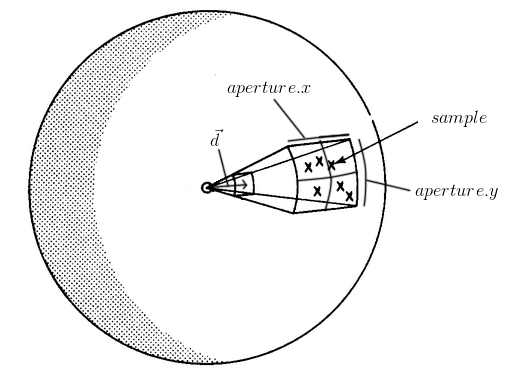
\includegraphics[width=0.5\textwidth]{img/conesampler.png}
	\end{center}
	\caption{Shéma du \emph{ConeSampler}}
\end{figure}

L'introduction du \emph{ShaderManager} a été très utile. C'est l'objet qui va gérer tous les
shaders utilisés dans le projet.

\section{Diagramme de classe}

Pour posséder une cohérence dès le début et tout au long du projet, un diagramme
de classe a été crée.

\begin{figure}[h]
	\begin{center}
		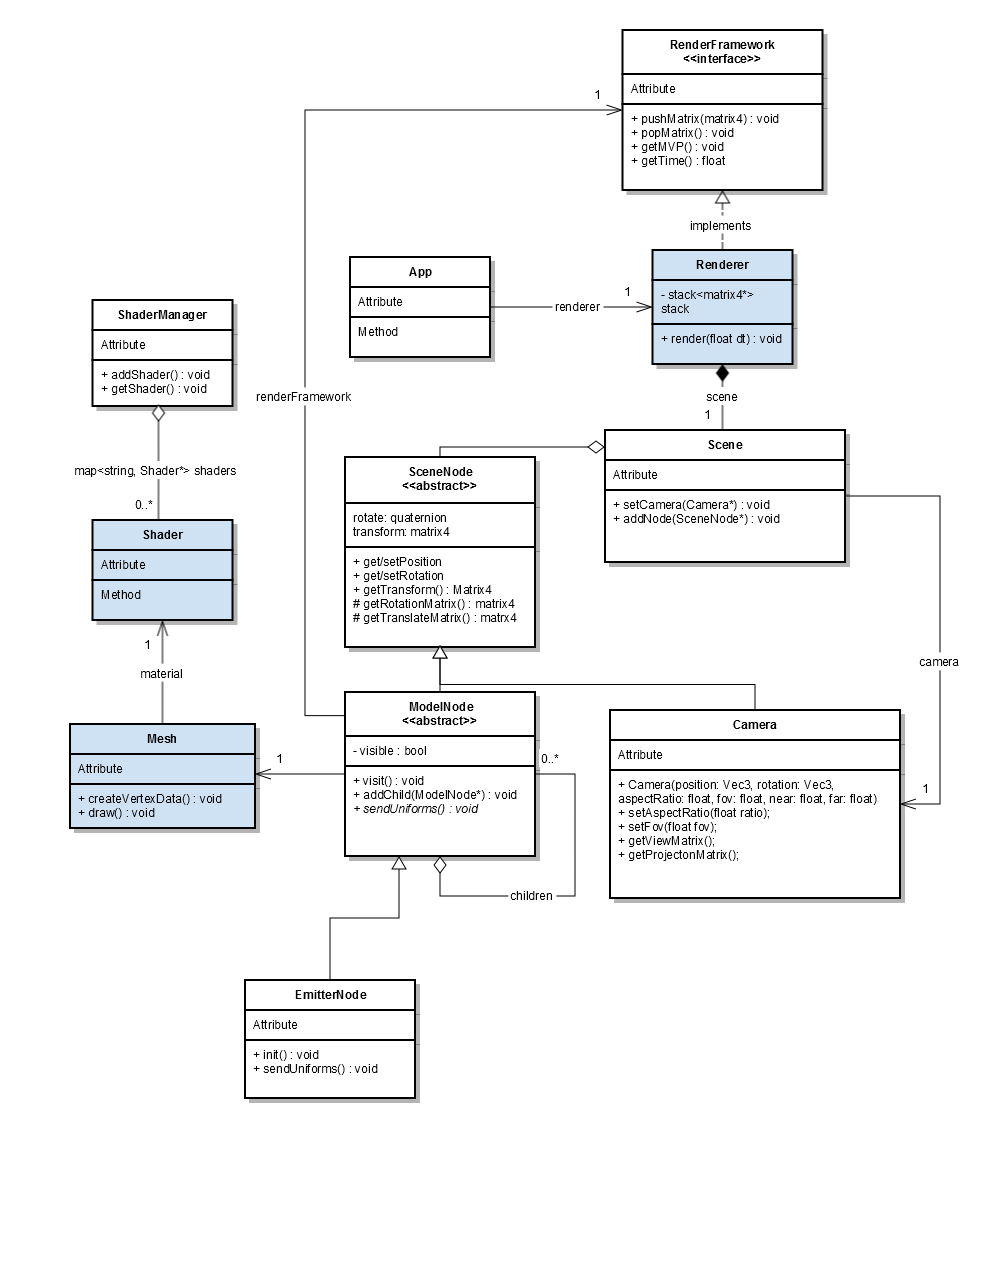
\includegraphics[width=0.9\textwidth]{img/UML.png}
	\end{center}
	\caption{Diagramme UML du projet}
\end{figure}

\newpage

\section{Structure de données}

Comme évoqué précédemment, toute la partie physique des particules est gérée via
des shaders. Ceux-ci récupèrent plusieurs données dans le buffer. Chaque
élément de ces données va représenter un attribut d'une particule. Ainsi,
celles-ci sont définies par une position, une couleur, une vitesse, un
\emph{timer} de vie et une durée de vie. Ces cinq attributs sont présents dans
les shaders, et une \emph{struct} est existante dans la classe
\emph{EmitterNode}.

\begin{figure}[h]
	\begin{minted}[bgcolor=bg]{c}
struct EmitterVertexData {
    Vec3 position;
    Color color;
    Vec3 velocity;
    float delay;
    float lifetime;
};
	\end{minted}
	\caption{Structure \emph{EmitterVertexData}}
\end{figure}

